
\chapter{Data analytics}

In this chapter I propose three hypotheses, each to be supported by analysis in the coming sections. The hypotheses are:

\begin{enumerate}
  \item Skedge's differences from and additions to CDCS are \textbf{usable and have real need}.

  \item Skedge’s \emph{navigations-per-add} demonstrate its \textbf{effectiveness} in the user search paradigms of \textbf{a) direct search} and \textbf{b) exploratory search}.

  \item \textbf{SkedgeQL is user-friendly}; users learn how to make more sophisticated search queries over time \textbf{simply by using it}.
\end{enumerate}


\section{Usage}

In this section, I will address many of the features listed in Chapter 2 (Design) and demonstrate their usability. To date, Skedge has seen\ldots

\vspace{5pt}

\begin{center}
\begin{tabular}{l}
  \hline
  4,713 users that have added or bookmarked at least one course \\ 
  5,256 schedules, with an average of 5.13 and median of 5 sections per schedule \\ 
  75\% of sessions from returning visitors \\ 
  107 sessions averaged per day \\ 
  5.4 pages viewed averaged per session  \\ 
  6 minutes spent averaged per session \\ 
  \hline
\end{tabular}
\end{center}

\noindent The figure of 4,713 total users may be misleading because, as explained in Chapter 3, if a user resets their browser cookies or changes browsers or devices, this registers as a distinct visitor. Unfortunately, even analytics tools that track unique visitors rely on cookies as well.

In an attempt to exclude ``stale users,'' we can time-constrain our analysis. In the past month, there were 1,416 visitors to the site and 672 visitors \emph{with schedules}. However, this metric excludes data from seniors who did not have need for Skedge in the past month. Going back to November 3, 2015, course registration day ($\sim$5 months ago), we find 4,647 visitors to the site and 1322 visitors with schedules. Thus, we can estimate that the amount of users who have added courses with Skedge is about \textbf{one-fifth} of all undergraduates (6,046) at the College.

\subsection{Search}

\begin{figure}[H]
  \centering

  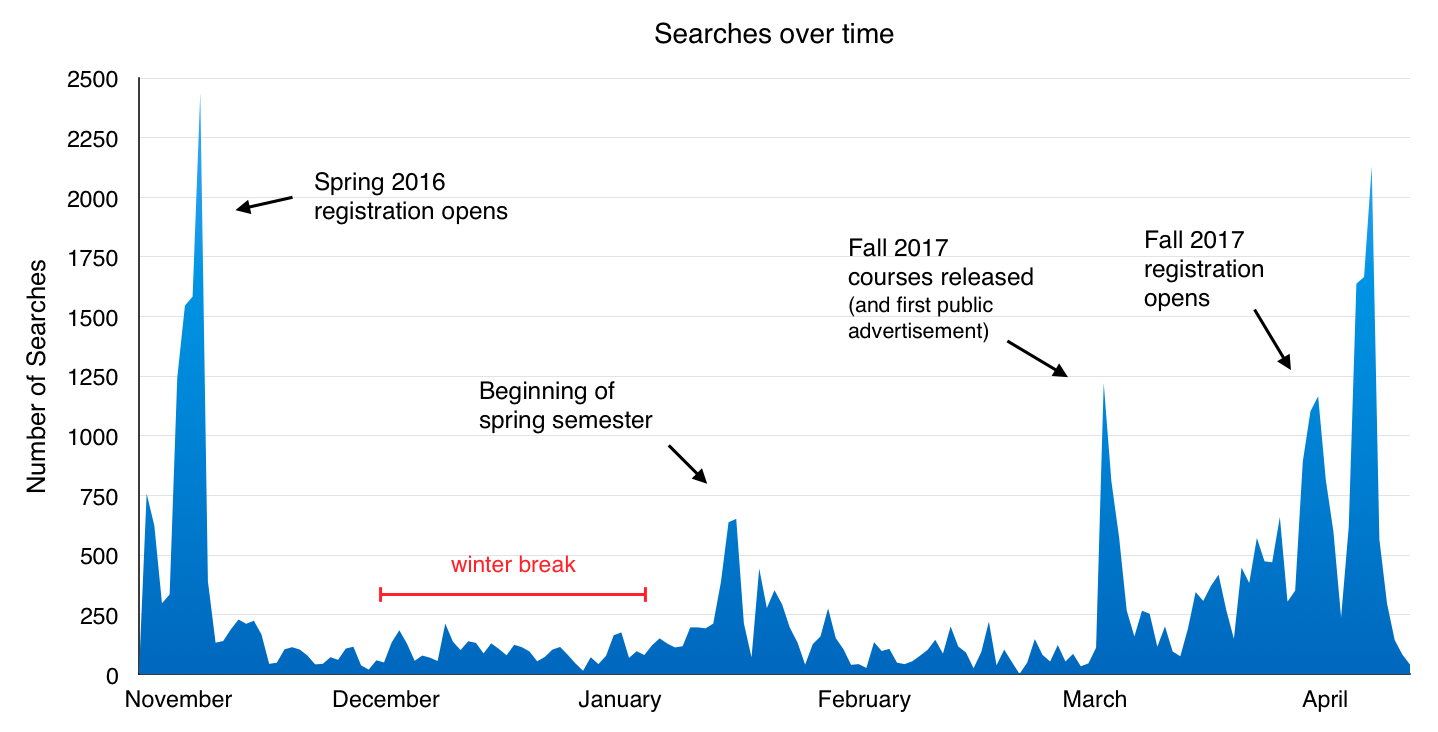
\includegraphics[width=1.0\textwidth]{images/graph/searches}

  \caption{Searches over the period Oct 19 2015 to Apr 11 2016, annotated with major events}
  \label{fig:searches}

\end{figure}

Figure \ref{fig:searches} shows searches over time, and makes the periodicity of Skedge usage extremely apparent. Although there is only enough data for a bit more than one ``phase,'' the cycle of events---\emph{semester begins} (students check course times, room locations, etc. while they get accustomed to the semester), \emph{next semester's course catalog released} (students explore the courses offered and build possible schedules), \emph{next semester registration opens} (cross-checking and officially registering each course with the Registrar)---clearly drives the majority of site traffic.

What this means is that Skedge is not seen as an experiment or a proof of concept that is not production-ready. Rather, its traffic patterns show that it is consistenly \emph{relied upon} by students and used for its intended purpose in times of biggest course scheduling need.

It should also be noted that before March, the majority of the userbase as I knew it consisted of seniors, as the majority of people that I knew personally and shared Skedge with belonged to my class. The latest two major events reported in the graph above thus very impressively consist of \emph{very few seniors}, who have no courses left to schedule. March also marked the very first time I publicly advertised Skedge, although not very strongly. It was sent out to all students in the Computer Science mailing list as well as posted to two class-wide Facebook groups.

The usability of and user satisfaction with a tool is hard to measure when it holds a monopoly. Considering that Skedge is an \emph{optional alternative} to CDCS, such consistent usage data (especially with 75\% of sessions being from returning users) undeniably prove its measures of usability and user satisfaction relative to CDCS.

  \subsubsection{Search types}

  \begin{figure}[H]
    \centering
    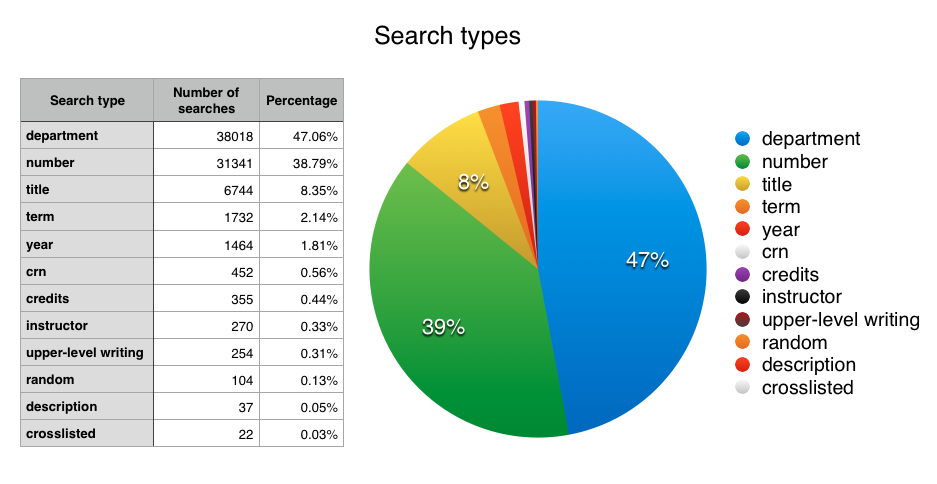
\includegraphics[width=1.0\textwidth]{images/graph/searchtypes}

    \caption{Breakdown of search queries by type of search}
    \label{fig:searchtypes}
  \end{figure}


Figure \ref{fig:searchtypes} validates the hypothesis made in Section 2.3 regarding the search interface design, demonstrating that the \emph{department code} and \emph{course number} search modes dominate user searches, accounting for over 85\% of all searches on Skedge. Bringing the nondistinct field for this in CDCS into prominence is thus a design choice that accomodates empirical behavior.

\subsubsection{Empty searches}

  Of the total 45,466 searches on Skedge logged since November 2nd 2015, 89.4\% (40,625) of searches produce nonempty search results, whereas 10.6\% (4,841) of searches come up empty.

  This already is evidence of an effective search mechanism, but of those empty searches, the vast majority contain typos or are for courses that simply don't exist. The other significant portion of searches include instructor names without the requisite ``taught by'' for SkedgeQL to pick it up as an instructor search, and this issue could easily be fixed.

  This type of analysis is powerful, as it can raise issues in the query language (i.e. searches I didn't implement but that users expect to work) with specific fixes. This is the same method WolframAlpha describes its team using to improve their freeform input system \cite{wolfram2}. Table \ref{fig:empty-queries} lists a few notable examples of this nature. (Table \ref{fig:funny-queries} lists a few funny queries I came across.)

\subsection{Exports}

In Section 2.2.5 (on the design of Skedge's schedule exporting), a major usability improvement claimed was the ability to export schedules to the {\tt .ics} format, a widely used format for many calendar applications, as well as offering functional Google Calendar export. Figure \ref{fig:exports} shows usage of the export functions over time, demonstrating its consistent and healthy use (traffic surges once again in line with major scheduling events.) This data confirms that there is strong demand for exporting to {\tt .ics}---it is even more common than Google Calendar export.

\subsection{``Link-searches''}

Figure \ref{fig:linksearches} shows the amount of clicks on the Wikipedia-style embedded links throughout Skedge (instructor names link to other courses they are teaching, prerequisite and crosslist course mentions link to those courses). The number of manual instructor searches is also included for comparison, which can be seen to be vastly less usable than the analogous link-click, which doesn't exist in CDCS. Additionally, link-clicks also possibly offer a different functionality (e.g. in the course browsing paradigm).

\singlespacing
{\renewcommand{\arraystretch}{1.75}
\begin{center}
\begin{table}[H]
\vspace{5pt}
  \begin{tabular}{ p{6cm} p{7.5cm} }

    {\large Empty search examples}
    & {\large Specific fix to SkedgeQL required} \\

    \hline
  \hline

    ``{\tt Prereq 280}'' \newline ``{\tt has-Prereq: 280}''
    & Course dependencies \\ \hline

    ``{\tt tuesday 3:25-4:40}'' \newline ``{\tt m/w}'' \newline ``{\tt classes tuesdays and thursdays between 11:05 and 12:20}'' \newline ``{\tt weekend summer 2016}''
    & \parbox[c]{\hsize}{Better day-of-the-week handling} \\ \hline

    ``{\tt 2 credits natural science}'' 
    & Search by division (although there were very few) \\ \hline

    ``{\tt religion and classics}'' \newline ``{\tt studio art}'' 
    & Search by full department name \\ \hline

    ``{\tt new csc courses}'' 
    & The word ``{\tt courses}'' stimies the query here (somewhat common with advanced query types) \\ \hline

    ``{\tt curriculum change}'' 
    & Alternative for ``{\tt new}'' keyword \\ \hline

    ``{\tt guo}'' 
    & Instructor without ``{\tt taught by}'' (very common) \\ \hline

    ``{\tt stt212 vs mth201}'' \newline ``{\tt stt212 OR mth201}'' \newline ``{\tt csc 2\{4,8\}2}'' \newline ``{\tt csc 242|282}''
    & Searching multiple queries at the same time \\ \hline

    ``{\tt crosslisted csc lin}'' 
    & Probably a more reasonable syntax than the current SkedgeQL one (``{\tt csc x lin}'') \\ \hline

    ``{\tt place: hubbell}'' \newline ``{\tt hubbell friday}'' 
    & Search by location, although motives unclear \\ \hline

    ``{\tt MTH 2*}'' \newline ``{\tt csc 2xx}''
    & Using ``{\tt *}'' or ``{\tt x}'' instead of an omission (e.g. searching ``{\tt MTH 2}'' would work for this purpose) \\ \hline

  \end{tabular}
  \caption{Example of search queries that produced no results but that indicate demand for added search features. The corresponding features that currently lack in SkedgeQL are described on the right.}
  \label{fig:empty-queries}
\end{table}

\vspace{5pt}

\begin{table}[H]
  \centering
  \begin{tabular}{ l l l }

    \hline

    ``{\tt why 123}''
    & ``{\tt taught by seligman}''
    & ``{\tt cool stuff}''
    \\ 

    ``{\tt psy cool professor}''
    & ``{\tt interesting courses}''
    & ``{\tt fun classes in csc}''
    \\ 

    ``{\tt easy A}''
    & ``{\tt flute birdman}''
    & ``{\tt how do i make a new schedule}''
    \\ 

    \hline

  \end{tabular}
  \vspace{10pt}
  \caption{A sample of some funny searches}
  \label{fig:funny-queries}
\end{table}
\end{center}

\doublespacing

\begin{figure}[H]
  \centering
    \begin{subfigure}[w]{14.5cm}
      \centering
      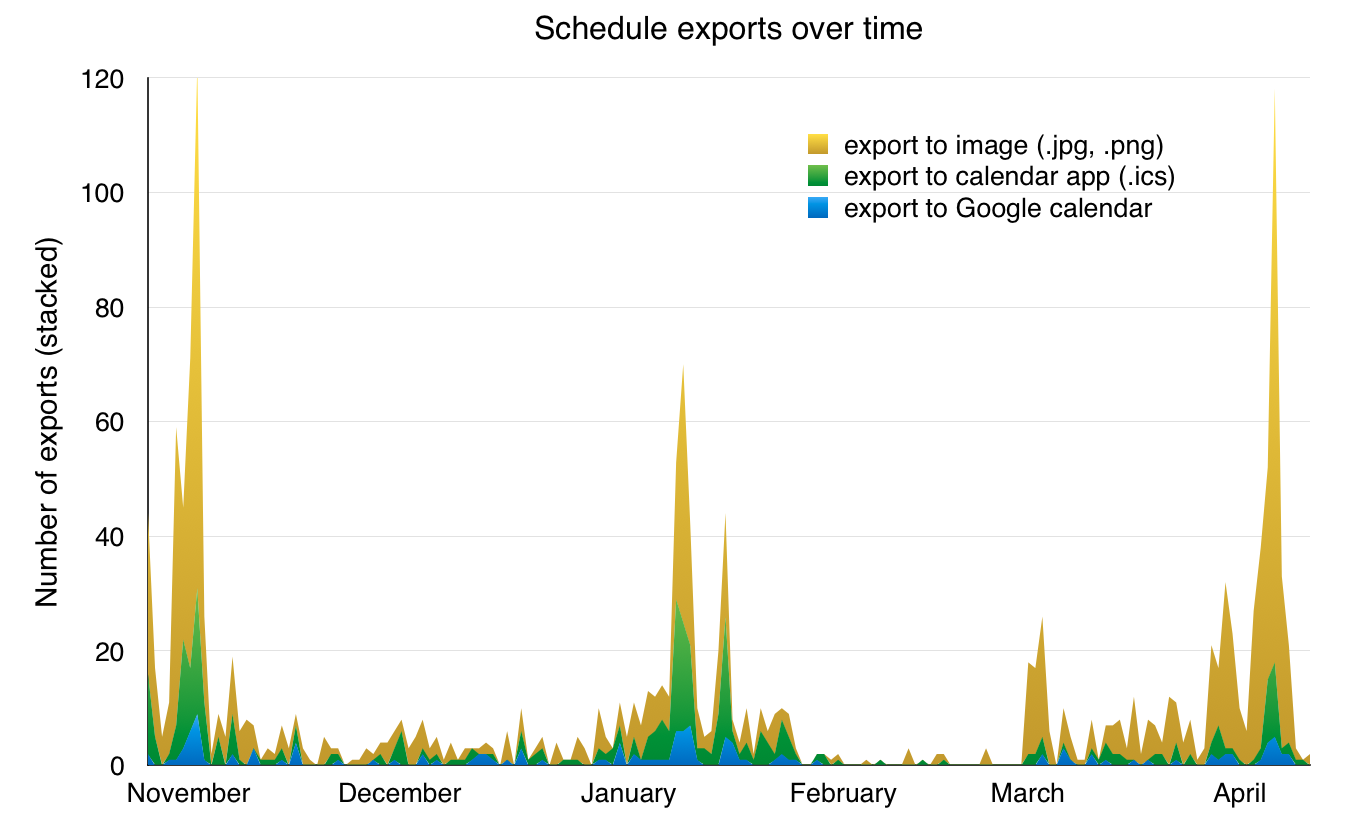
\includegraphics[width=1.00\textwidth]{images/graph/exports}
      \caption{Different types of schedule exporting over time} \label{fig:exports}
    \end{subfigure} \\

    \vspace{30pt}

    \begin{subfigure}[w]{14.5cm}
      \centering
      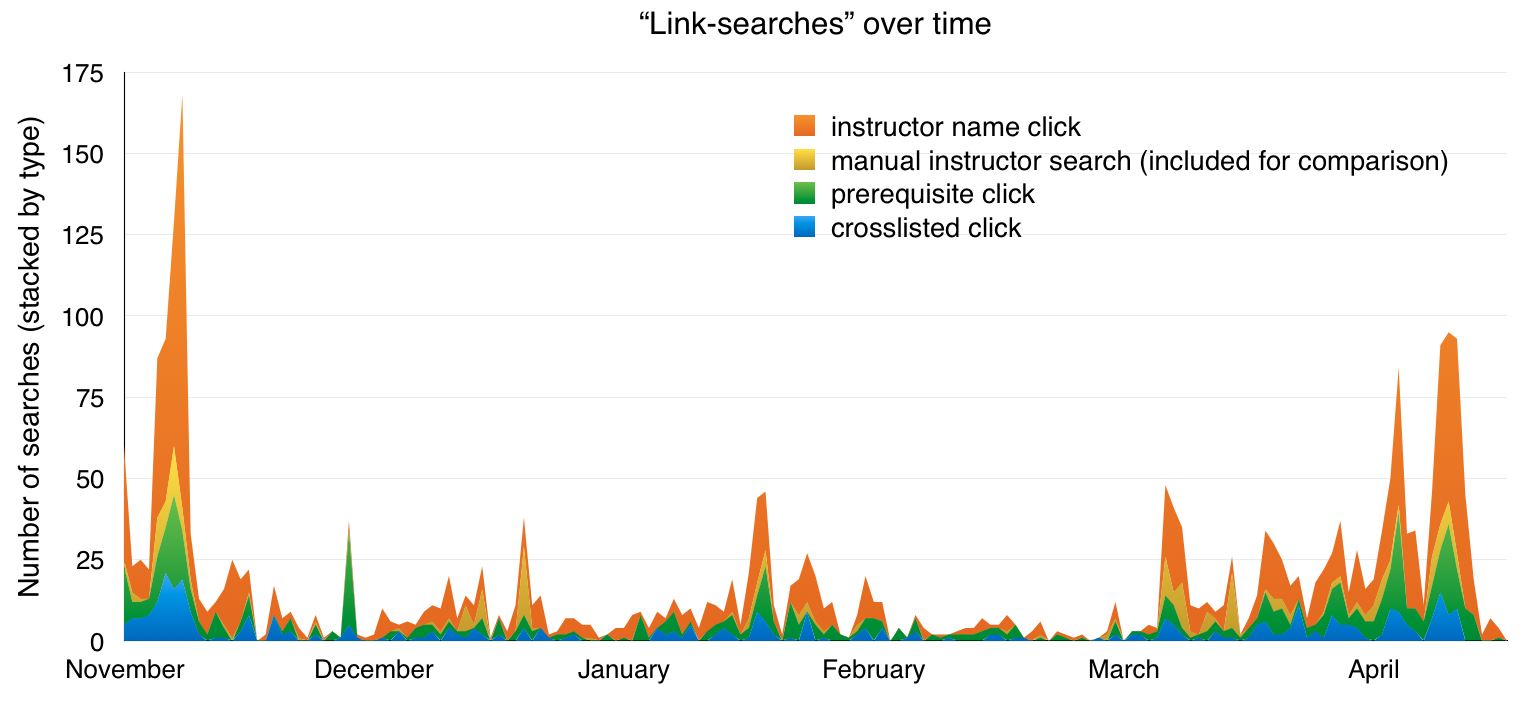
\includegraphics[width=1.00\textwidth]{images/graph/linksearches}
      \caption{Different types of ``link-search'' clicks over time, with manual instructor search included for comparison with clicking on an instructor's name} \label{fig:linksearches}
    \end{subfigure}

  \caption{Other metrics of Skedge usage over time}
\end{figure}

\clearpage

\subsection{Mobile}

Making the case for usability superior to CDCS's in the space of mobile support is easy, given that CDCS does not have a mobile-responsive website. But to illustrate the importance of ensuring good user experience on mobile devices, consder that 11.54\% of all Skedge sessions are from mobile devices, which is very substantial. On average, 2.74 pages viewed are viewed and 2 minutes are spent per session on mobile devices.

The nature of the content also makes Skedge commonly accessed on the go---quickly looking up room numbers while heading to class, for instance, or checking a friend's schedule on Skedge Social to meet them after a class, etc. There is still work to be done to determine the usability of Skedge's mobile site in particular. Surveys could be a good indicator, but I didn't have the chance to administer any.

\subsection{Social}

Since March 1st (40 days), based on 963 sessions on {\tt /social}, Skedge Social has seen\ldots

{\renewcommand{\arraystretch}{1.5}
\singlespacing
\begin{center}
\begin{tabular}{l}
  \hline
  141 users have linked Skedge to Facebook \\
  10,242 page views (256 page views/day)  \\
  10 pages/session (users cycle through tabs and go back to it) \\
  a 5\% bounce rate (users interact with it) \\
  67\% of visits being were returning visitors \\
  284 overlays onto friends’ schedules (2 per user) \\
  \hline
\end{tabular}
\end{center}
\doublespacing

\vspace{5pt}

\noindent Although the feature is too young for in-depth data analysis, these initial reports show promise, especially in the rate of adoption (around 3.5 users per day on average), its level of interaction, and the rate of \emph{returning} users to Skedge Social.

\subsection{Course blocks}

\begin{figure}
  \centering

  \fbox {
    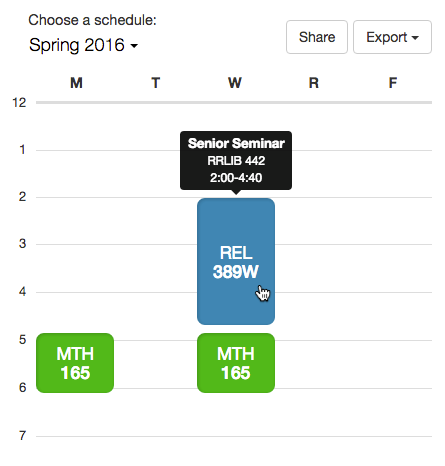
\includegraphics[width=6cm]{images/skedge/blocks}
  }

  \caption{Hovering over a course block in Skedge's side-schedule shows at-a-glance information about it; clicking on it navigates the user to that course}
  \label{fig:searchtypes}

\end{figure}

As a user adds courses to their schedule, the courses appear as timeblocks on the schedule to the side of the search results. The blocks only display the course code (i.e. department code, course number, and if it is a subsection such as a lab or workshop), but hovering over them displays more useful information like the course title, location, and the exact start and end times.

Interestingly, the only course information that is gained by clicking on courses is the description, instructor, and perhaps minor details like course comments, prerequisites, etc. Yet, of 12,944 sessions of users with schedules, \textbf{40\%} of those sessions had at least one block-click. Those sessions with block clicks averaged \textbf{5.12 block-clicks per session}, a strikingly high number considering its limited functional use! How do we explain this?

I hypothesize that a combination of Skedge's presentation of information, highly interactive user interface, and concern for quality of user experience contributes to a sense of enjoyment in course scheduling. Five clicks corresponds to five courses (both the median and mean for sections per schedule is 5), meaning that in every session, a user could be reviewing details and reading over descriptions for each of their courses. Enabling this sense of pride and admiration with one's course selection is a crucial aspect of Skedge's mission. I believe the courses one chooses to take are an integral aspect of one's personal development and outlook on life in college. I believe ensuring that students are excited not only about their courses, but also about \emph{exploring} what their university has to offer is key to an inspired, intellectually curious student body.

The above could only be confirmed with involved user studies, for which I have no data. At the very least, the average block-clicks per session is a strong case for Skedge's usability over CDCS for the simple reason that Better CDCS does not even allow users to click on their schedule blocks, and this usage data shows that there is clearly a desire to do so.
\clearpage

\section{Effectiveness of search}

\subsection{Definitions}

A navigation is defined as
a search, or
a click on an instructor’s name, or
a click on a crosslisted or prerequisite course link

The navigations-per-add measure is
the number of navigations a user took (within one session) until a course was added, bookmarked

\subsection{Trends}

\begin{figure}
  \centering
  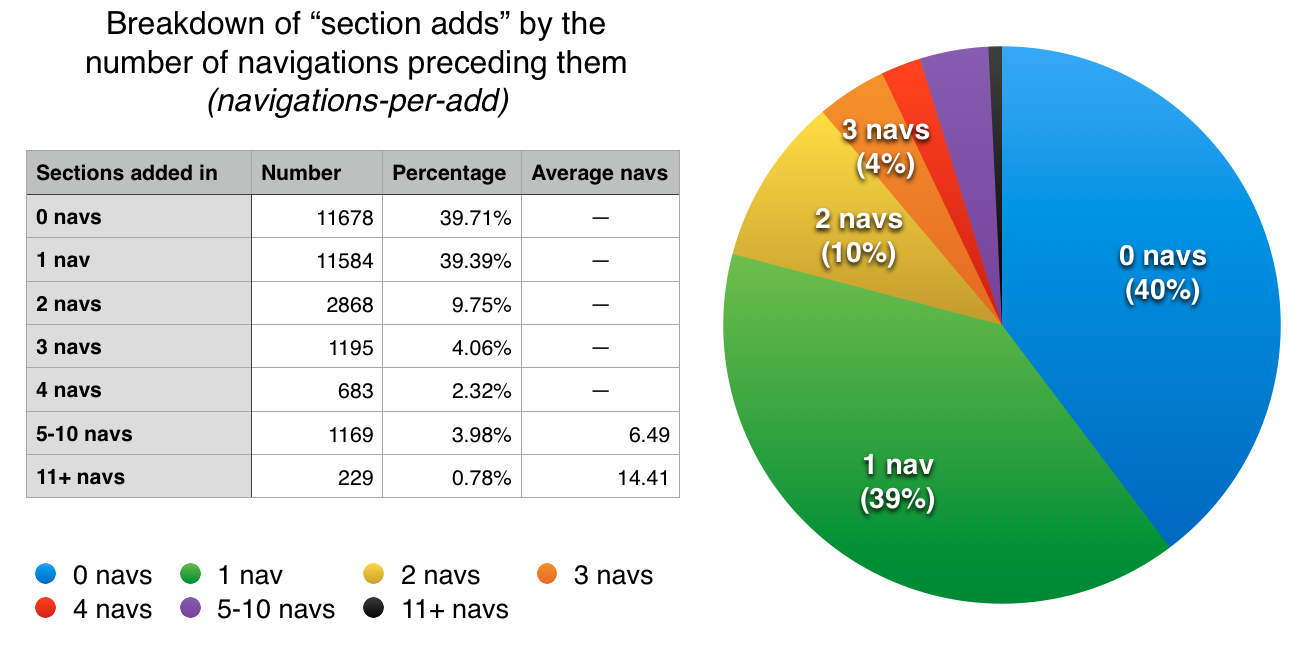
\includegraphics[width=1.0\textwidth]{images/graph/combined_navs}

  \caption{Etc}
  \label{fig:searchtypes}
\end{figure}

\subsection{Breaking them apart}

  behavioral patterns
  Direct search for specific course
  Discovery, browsing, exploring

  \subsubsection{Direct searches}

  \begin{figure}
    \centering
    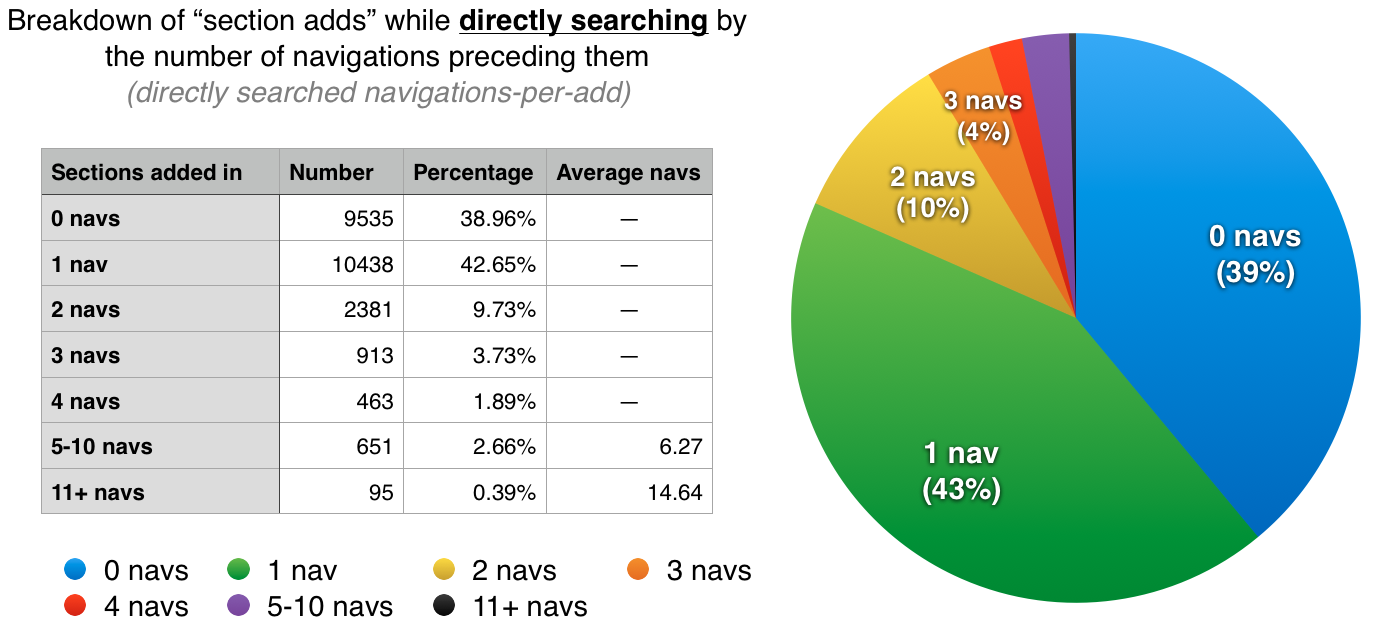
\includegraphics[width=1.0\textwidth]{images/graph/direct_navs}

    \caption{Etc}
    \label{fig:searchtypes}
  \end{figure}

  Why would 0-navs be so common with direct searches? 64\% of them subsections!

  \subsubsection{Browse}

  \begin{figure}
    \centering
    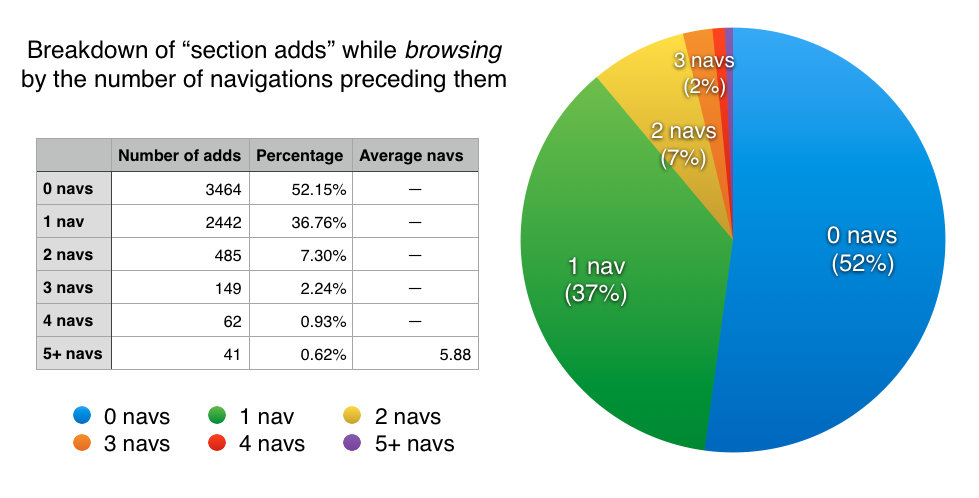
\includegraphics[width=1.0\textwidth]{images/graph/browse_navs}

    \caption{Etc}
    \label{fig:searchtypes}
  \end{figure}

  As expected, the 0-navs were mostly maincourses (62\%)

  Effective++

  \subsubsection{Social}

  90 users have linked Skedge to Facebook
  Since March 1st,
  4,000+ visits (200 visits/day)
  ~60\% of visits to /social were returning visitors
  90 overlays onto friends’ schedules
  10 clicks to Facebook profiles :(
  - get stats from the fb dashboard

  success?????
\clearpage


\section{Complexity of users' searches over time}

\subsection{Definitions}

The \textbf{complexity} of a search query is the number of fields that aren't course number or department that it spans (the accepted fields are shown in Table \ref{fig:sc-fields}).

\singlespacing
\begin{center}
\begin{table}[H]
  \centering
  \begin{tabular}{ lllll }

    \hline

    description
    & title
    & credits
    & crosslisted
    & CRN
    \\

    
    instructor
    & year
    & term
    & upper-level writing
    & random
    \\

    \hline

  \end{tabular}
  \vspace{10pt}
  \caption{``Complex'' search fields (omits only number and department)}
  \label{fig:sc-fields}
\end{table}
\end{center}
\doublespacing

\noindent We can compute the number of searches it takes a user to reach a new highest search complexity record since the previous record. See Table \ref{fig:sc-example} for an illustrative example.

A user's \textbf{first increase in search complexity} is defined as the number of searches a user made before searching with complexity greater than zero. If a user's first search has complexity 1, the user's \emph{first increase} is 0.

A user's \textbf{second increase in search complexity} is defined as the number of searches a user made before searching with complexity greater than their \emph{first increase}'s search complexity.

It is possible that user have neither, both, or only a \emph{first increase} metric.

{\renewcommand{\arraystretch}{2.0}
\singlespacing
\begin{center}
\begin{table}[H]
  \centering
  \begin{tabular}{ r | c c c | l }

    Query no.
    & Search query
    &
    & Complexity
    & Searches till increase \\

    \hline

    \#1
    & ``{\tt CSC}''
    & \rightarrow
    & 0
    & 
    \\

    \#2
    & ``{\tt MTH 165}''
    & \rightarrow
    & 0
    & 
    \\

    \#3
    & ``{\tt csc taught by guo}''
    & \rightarrow
    & 1
    & $3-1=\textbf{2}$ \hspace{2pt} \emph{(first increase)}
    \\

    \#4
    & ``{\tt random mur 1-2 credits}''
    & \rightarrow
    & 2
    & $4-3=\textbf{1}$ \hspace{2pt} \emph{(second increase)}
    \\

  \end{tabular}
  \vspace{10pt}
  \caption{Illustration of computing the number of searches before a complexity increase}
  \label{fig:sc-example}
\end{table}
\end{center}
\doublespacing


\subsection{Motivation}

The purpose of this metric is to determine the usability and learning curve of SkedgeQL. The two ways Skedge currently offers to teach users about its query language are

\begin{enumerate}
  \item  by providing a table of example queries whenever the user clicks inside the search field from the Skedge homepage (see Figure \ref{fig:sk-search2}), and

  \item  from embedded links on the site making searches with high complexity and implicitly demonstrating them to users by using the same input field they use to submit searches.\footnote{Clicking on an instructor's name, for instance, makes the advanced search ``for the user.'' Another example is clicking on a course box in the side schedule, which searches for that course code along with its term and year (e.g. ``{\tt CSC 171 Fall 2016}'').

  Other possibilities include linking the credits field of each course to a credits search, the CRN field of a section to a CRN search, the ``{\tt W}'' part of the course code to an upper-level writing search, having a crosslisted course link search the crosslisting of the two departments (instead of directly link to the crosslisted course), a ``feeling lucky?'' button for a search with ``{\tt random}''.}
\end{enumerate}

\begin{figure}[H]
  \centering
  \fbox{
    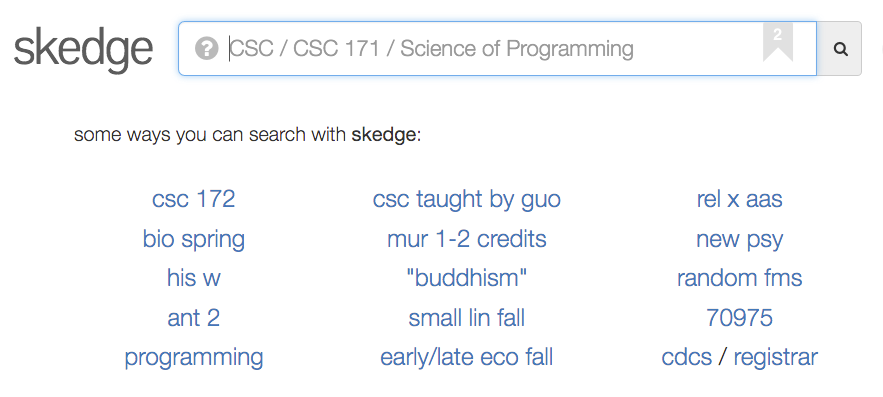
\includegraphics[width=0.65\textwidth]{images/skedge/search}
  }
  \caption{Examples of SkedgeQL} \label{fig:sk-search2}
\end{figure}

\noindent The latter method is, of course, much preferred to the former as it teaches without requiring concerted effort on the part of the user to study and learn the query language, and mostly likely remains more memorable and intuitive as a result.

A \emph{high} percentage of users with \emph{first increase} and \emph{second increase} metrics, with \emph{low} mean and median values for those increases would be desirable. This would strongly indicate the effect of teaching method \#2 because the factor in teaching users about the query language would simply be time (besides the case of users becoming curious about advanced search types and looking them up explicitly, which is difficult to account for because the query example box is shown to all users fairly regularly).

\subsection{Trends}

\begin{figure}
  \centering
  \vspace{-10pt}

  \begin{subfigure}[w]{0.85\textwidth}
    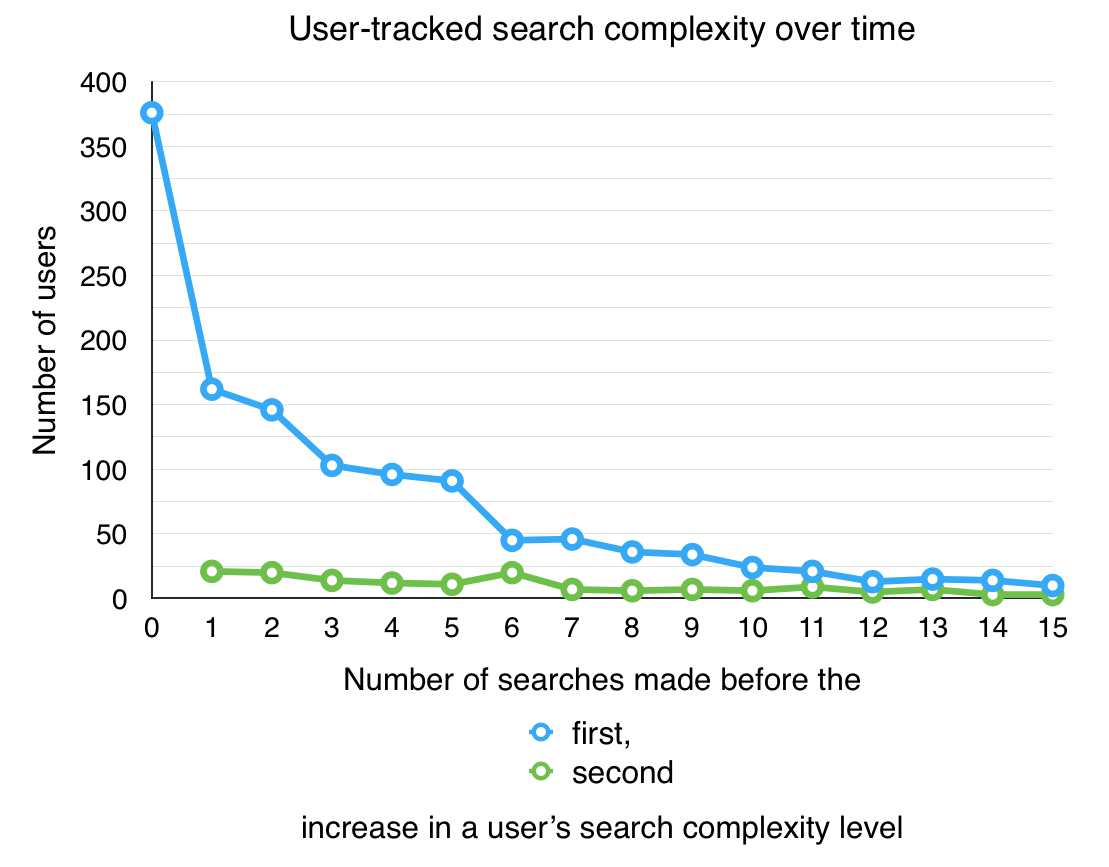
\includegraphics[width=1.00\textwidth]{images/graph/search_dt}
    
    \caption{Etc}
    \label{fig:sc-graph}
  \end{subfigure}

  \\
  \vspace{30pt}

  \begin{subfigure}[w]{0.75\textwidth}
    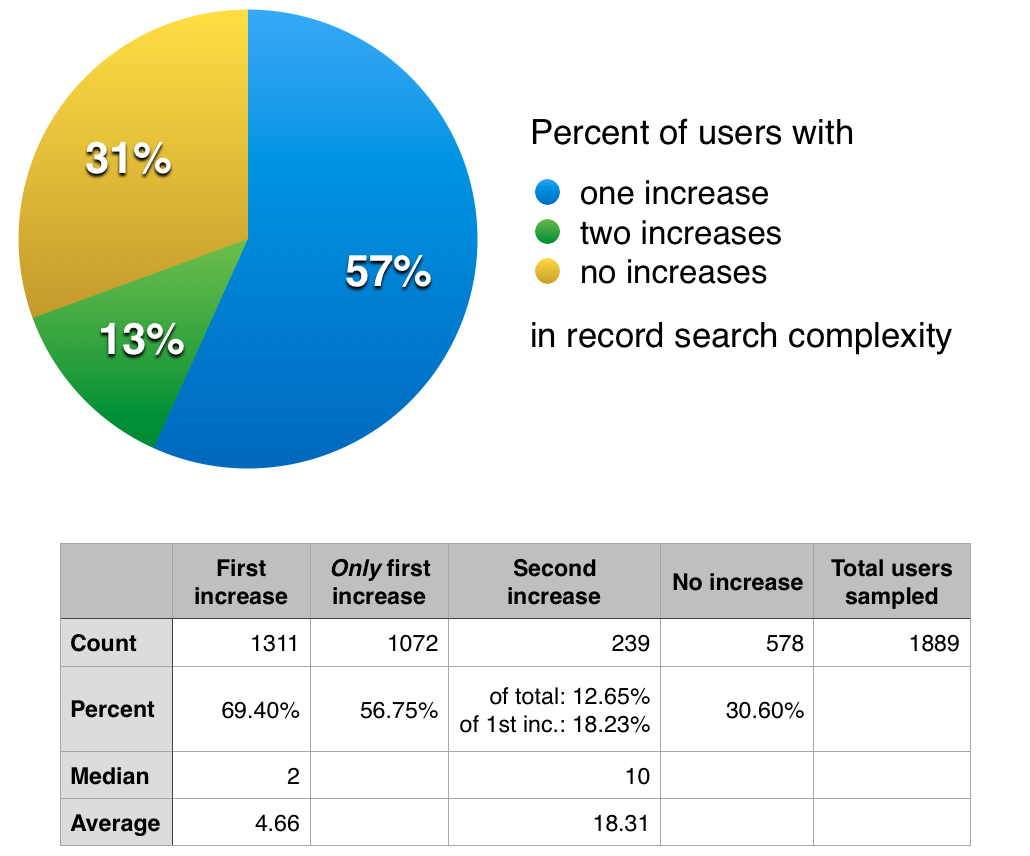
\includegraphics[width=1.00\textwidth]{images/graph/search_dt_pie}

    \caption{Etc}
    \label{fig:sc-pie}
  \end{subfigure}

  \caption{Etc}
\end{figure}

The blue line in Figure \ref{fig:sc-graph} plots the number of users 

First increase 69.4\% of users), with a median of 2 searches.
Note that starting at search complexity one or greater counts as a ``searches before first increase value'' of 0.

Second increase (7.9\% of users)
Median: 8 searches
Average: 17.52 searches

DSQL++
\clearpage

